% Suggested sentence for the main experimental setup:
% For INSIDE-Coalition, we use K=64 and the normalized weight lambda=1/16;
% sensitivity analyses are reported in Appendix~\ref{app:inside_sensitivity}.

\subsection{Sensitivity to the moment weight and candidate-pool size}
\label{app:inside_sensitivity}
We conduct a one-at-a-time sensitivity analysis on the 100-player Airport
game at a fixed budget of 50,202 utility calls, comprising 50,000 interior
queries and 202 boundary queries. We vary
$\lambda\in\{1/64,1/32,1/16,1/8,1/4,1/2,1\}$ with $K=64$, and
$K\in\{8,16,32,64,128\}$ with $\lambda=1/16$.
Here $\lambda$ denotes the normalized input weight used in our implementation;
the corresponding coefficient in the unnormalized first-moment score is
$\lambda(n-2)/(n-1)=98\lambda/99$ for Airport.
All settings share the coalition-size schedule and player relabeling within
each of three repeats and use the same strict conditional-mean estimator.
Changing $K$ does not require nested candidate pools. The common default
is evaluated once per repeat, giving 33 designs in total.
We compute RMSE against the exact Shapley values and use the equal-size
first- and second-moment discrepancies $D_1$ and $D_2$ defined above.

Increasing $\lambda$ from $1/64$ to $1$ reduces mean $D_1$ from $0.02566$
to $0.006016$, while increasing mean $D_2$ from $0.02776$ to $0.03458$.
This illustrates the intended tradeoff between the two moment objectives.
Mean RMSE at $\lambda=1/32,1/16,1/8$ is respectively
$0.005145$, $0.005457$, and $0.005494$; the largest is approximately
$6.8\%$ above the smallest. Thus, the default is not an isolated optimum
in this neighborhood. This observation is descriptive and does not
establish statistical equivalence or robustness across all games and budgets.

Larger candidate pools reduce the observed moment discrepancies, but RMSE
is not monotone over $K=8$--$64$. Increasing $K$ from $64$ to $128$ reduces
mean RMSE from $0.005457$ to $0.004703$ (approximately $13.8\%$), while
increasing mean design time from $6.03$ to $10.72$ seconds
(approximately $77.9\%$). These results quantify a computation--accuracy
tradeoff; they do not establish accuracy saturation at $K=64$ or superiority
of this default over every smaller pool. We retain the pre-existing defaults.

\begin{figure}[t]
\centering
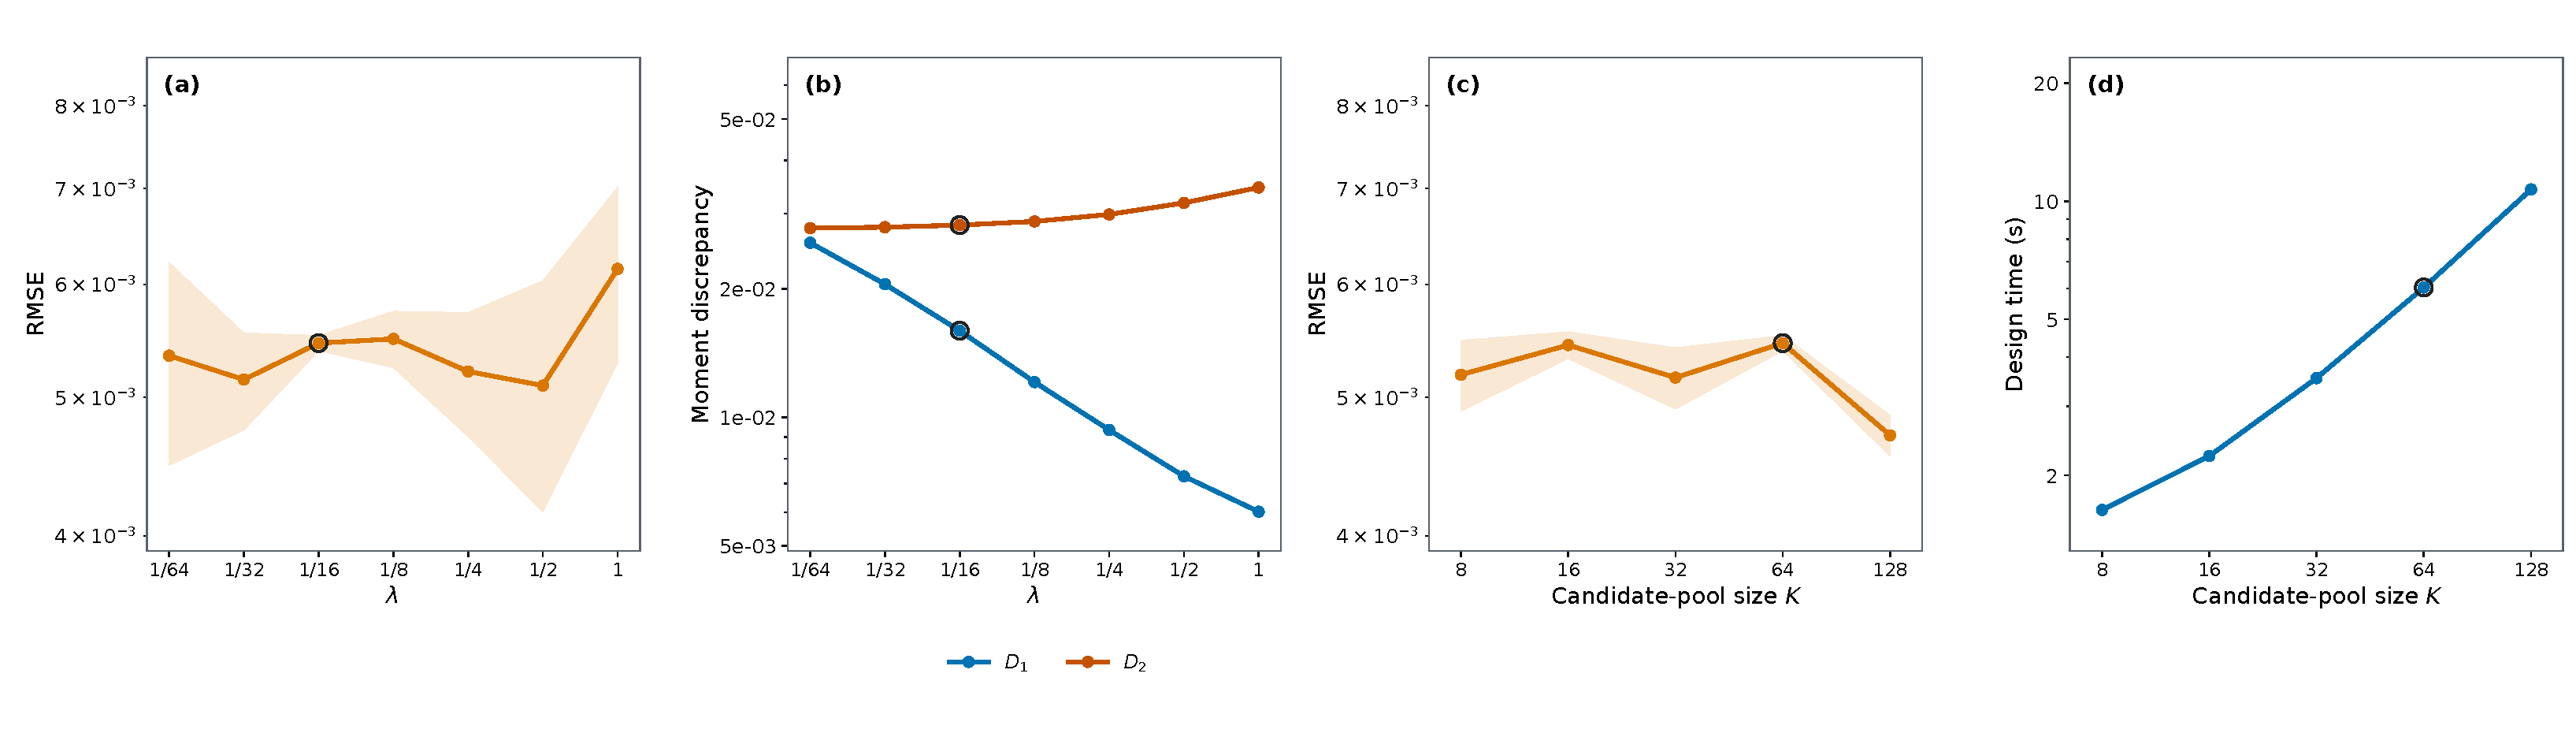
\includegraphics[width=\textwidth]{results/pdf/airport_inside_sensitivity.pdf}
\caption{Sensitivity of INSIDE-Coalition on Airport at a fixed utility-call
budget. (a) RMSE versus $\lambda$ with $K=64$.
(b) First- and second-moment discrepancies versus $\lambda$.
(c) RMSE versus candidate-pool size $K$ with $\lambda=1/16$.
(d) Design-construction wall time versus $K$.
Lines show means across three estimator seeds, and shading indicates
$\pm$ one sample standard deviation (denominator $3-1$).
Black rings mark the pre-existing defaults. All axes are logarithmic;
the RMSE panels share vertical limits. Timing uses 16 worker processes
with one BLAS/OpenMP thread per process. Configurations run sequentially
in a fixed randomized order; measured time includes worker startup and
excludes moment diagnostics, utility evaluation, and Shapley estimation.
Some standard-deviation bands are narrower than the plotted lines.}
\label{fig:inside_sensitivity}
\end{figure}
